\clearpage
\section{Hola Mundo!!!} \label{sec:hello}

El \emph{Hola Mundo} (o \emph{Hello World}) es la primera aplicación que típicamente se programa a la hora de aprender una nueva tecnología. Su funcionamiento es sencillo, imprimir por pantalla (o por el dispositivo de salida correspondiente) el saludo que da nombre a la aplicación. Con esta práctica se abordará la creación de un nuevo proyecto. También se creará una pequeña página para la que trabajaremos sobre el código \gls{HTML} de la aplicación. Veremos como probar la aplicación usando el navegador (Chrome en nuestro caso) de la máquina de desarrollo que utilizamos para desarrollar. Por último, haremos una primera aproximación a la característica de \emph{Data Binding} de Angular uniendo dos elementos del \gls{HTML} que aparecerán por pantalla.

Para crear nuestro primer proyecto, abrimos el PowerShell de Windows (o la consola de comandos tradicional, según disponibilidad y gustos personales) y nos dirigimos a nuestro directorio de trabajo. Aquí se creará el directorio que contendrá nuestro proyecto. En este caso queremos un proyecto en blanco, usando la plantilla \emph{blank}, para ello ejecutaremos el siguiente comando:

\begin{lstlisting}[language=bash]
  # ionic start HelloWorld blank --v2
\end{lstlisting}

Esto creará un directorio llamado HelloWorld dentro del cual veremos el proyecto sobre el cual vamos a trabajar.

\notebox{Con la opción \emph{--v2} indicamos que el queremos usar la versión de ionic para el nuevo proyecto.}

\begin{figure}[H]
\centering
  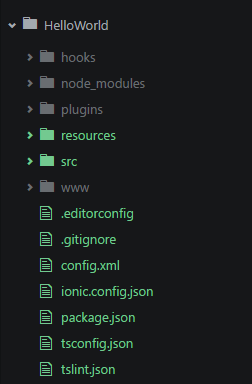
\includegraphics[height=0.4\textheight,keepaspectratio]{Figures/ch2/HelloWorld/atom_project_structure}
  \caption{Estructura del proyecto \emph{Hello World} al crearlo visto en Atom.}
\end{figure}

Podemos ejecutar la aplicación tal cual se encuentra en este momento y comprobar que funciona correctamente. Para esto, utilizando Ionic CLI, podremos ejecutar la aplicación sobre un servidor el cual servirá de servidor local para nuestra aplicación permitiéndonos acceder a ella a través de un navegador web:

\begin{lstlisting}[language=bash]
  # ionic serve
\end{lstlisting}

Tras unos segundos, nos aparecerá un mensaje indicando la \gls{URL} en la cual se encuentra disponible la aplicación. Por lo general, cuando el servidor termina de arrancar, se abrirá el navegador configurado por defecto en nuestro sistema apuntando directamente a la dirreción anterior. De no ser así, copiamos la \gls{URL} y la abrimos manualmente.
Vemos la página que por defecto viene con la plantilla utilizada.

\begin{figure}[H]
\centering
  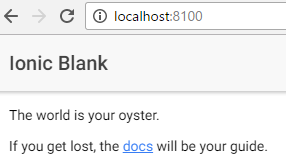
\includegraphics[width=0.4\textwidth,keepaspectratio]{Figures/ch2/HelloWorld/ionic_blank}
  \caption{Así es como se ve el template \emph{blank} al ejecutarse.}
\end{figure}

Vamos a editar la aplicación para que tenga el comportamiento antes indicado, es decir, que en nuestro caso es mostrar por pantalla el texto "Hello World!". Abrimos con el editor que vayamos a usar el fichero \emph{./src/pages/home/home.html}. Dentro de este fichero se encuentra el código de la página que acabamos de ver en el navegador.

\begin{figure}[H]
\centering
  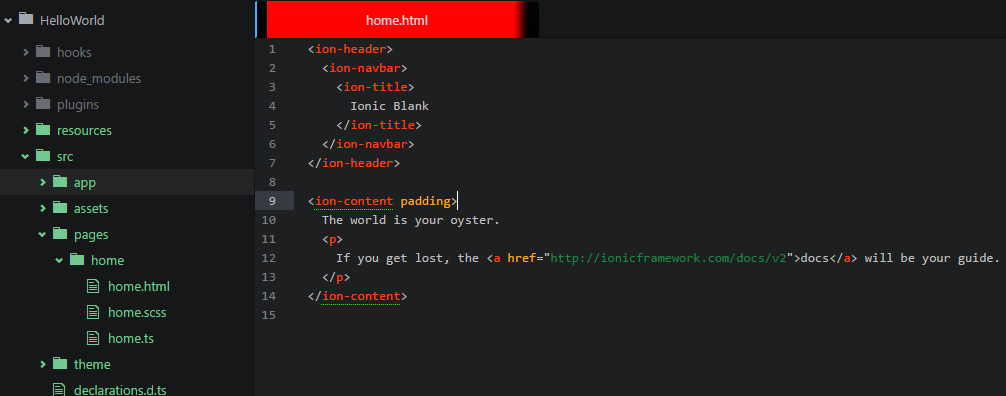
\includegraphics[width=\textwidth,keepaspectratio]{Figures/ch2/HelloWorld/home_ionic_blank}
  \caption{Página principal del template \emph{blank}.}
\end{figure}

\tipbox{Si utilizamos un editor un poco avanzado, nos ofrecerá la posibilidad de abrir un directorio de trabajo entero, pudiendo ver la estructura de ficheros de la aplicación y navegar fácilmente entre ellos.}

Podemos apreciar que la página dispone de una cabecera definida por el tag \emph{<ion-header>} y el cuerpo de la página definido por el tag \emph{<ion-content padding>}. Modificaremos el código de la siguiente manera:

\begin{lstlisting}[style=htmlcssjs,frame=tlrb,xleftmargin={0.2cm}]
  <ion-header>
    <ion-navbar>
      <ion-title>
        Hello App
      </ion-title>
    </ion-navbar>
  </ion-header>

  <ion-content padding>
    <p>HELLO WORLD!!!</p>
  </ion-content>
\end{lstlisting}

Una vez guardado el cambio, veremos en la ventana del PowerShell en la que hemos arrancada el servidor de Ionic que la aplicación se ha compilado de nuevo, y la propia página en el navegador se ha refrescado mostrando los cambios.

\begin{figure}[H]
\centering
  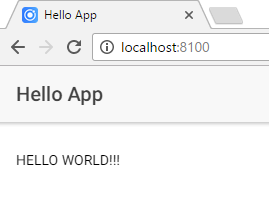
\includegraphics[width=0.4\textwidth,keepaspectratio]{Figures/ch2/HelloWorld/hello_world_1}
  \caption{Podemos ver nuestro Hello World en el navegador por primera vez.}
\end{figure}

Vamos a ir un poco más allá con nuestra aplicación. Para ello vamos a utilizar una de las características que nos ofrece Angular, el \emph{Data Binding}. Abrimos de nuevo el fichero \emph{home.html} y modificamos el cuerpo de la siguiente manera:

\begin{lstlisting}[style=htmlcssjs,frame=tlrb,xleftmargin={0.2cm}]
<ion-content padding>
  <ion-list>
    <ion-item>
      <ion-label color="primary" >My name is </ion-label>
      <ion-input [(ngModel)]="name" placeholder="your name" ></ion-input>
    </ion-item>
    <ion-item>
      <h1>Hello {{ name }}, nice to meet you.</h1>
    </ion-item>
  </ion-list>
</ion-content>
\end{lstlisting}

Con esta modificación hemos introducido un cuadro de texto, \emph{<ion-input>}, en el que podremos escribir nuestro nombre. También hemos cambiado el saludo, haciendo que este sea ``personalizado'' utilizando el valor introducido en \emph{\{\{ name \}\}}. Esto se consigue gracias a la potencia del \emph{Data Binding}. Si volvemos a ver nuestro input, vemos que uno de sus atributos es \textbf{[(ngModel)]}. Este atributo es una directiva de Angular que vincula un campo, el input en nuestro caso, con una propiedad del componente al que pertenece. Así, al declarar la directiva \emph{[(ngModel)]="name"}, hemos hecho que se cree una propiedad dentro del componente (si no la hemos creado manualmente editando el componente) y que su valor esté vinculado al del input. Ya solo nos queda utilizar este valor donde nos interesa utilizando la expresión \emph{\{\{ name \}\}}. Angular también se encarga de renderizar el valor cuando este cambia, por lo que a medida que vayamos escribiendo nuestro nombre, irá actualizándose la vista.

\begin{figure}[H]
\centering
    \centering
        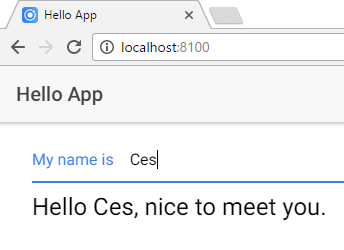
\includegraphics[width=0.3\textwidth]{Figures/ch2/HelloWorld/dyn_hello_world_1}
        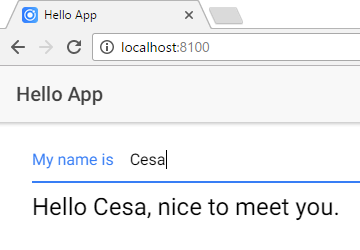
\includegraphics[width=0.3\textwidth]{Figures/ch2/HelloWorld/dyn_hello_world_2}
        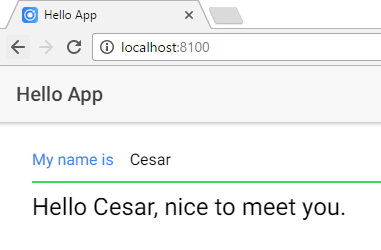
\includegraphics[width=0.3\textwidth]{Figures/ch2/HelloWorld/dyn_hello_world_3}
    \caption{Nuestra aplicación ahora nos ofrece un saludo dedicado.}
\end{figure}
